\section{Yarrawonga and Mulwala: Demand-responsive transportation in regional Victoria, Australia}
\label{sec:yarrawonga}
\hfill \textbf{Author:} Nicole Ronald
% ==================================================================================================================
In November 2013, Public Transport Victoria (PTV) implemented a service called
Flexiride in twin towns in regional Victoria, consisting of an on-demand public
transport service using taxis. This service replaced an existing fixed-route bus
service, which had a low patronage.

The aim of this scenario was to investigate the change in operational
performance between two different DRT schemes: the Flexiride scheme and a
completely ad-hoc scheme. More details can be found in
\citep[][]{RonThoWin2015}. This work is a first step towards developing a
decision-support tool to evaluate different DRT schemes, in particular
integrated with other modes of transport. 

% --------
%Associated projects: 
The scenario was built as part of a larger project exploring the viability of
mobility-on-demand, focusing on ridesharing and demand-responsive transportation
(DRT) services \citep[][]{Ronald_iMoD_2014}.

% --------
%Study area: 
The scenario covers twin towns on the border of Victoria and New South Wales,
Australia, separated by the Murray River. Yarrawonga (Victoria) has a population
of 7\,057 and an area of 95.0\,square kilometers, while Mulwala (New South Wales) has a
population of 1\,904 and an area of 18.6\,square kilometers. 

The Flexiride scheme delivers six services on weekdays and three services on
Saturday, leaving the center of Yarrawonga (Orr St) at fixed times.  The local
taxi operator is paid a holding fee by PTV to ensure that a taxi is available at
Orr St at the nominated time. The taxi returns to normal service if there are no
bookings and no passengers waiting.

Passengers can ride either by booking over the phone at least 10\,minutes before
the service is scheduled to depart from Orr St, or by arriving at Orr St in
person to begin their trip. Existing bus stops were used as pickup and dropoff
points.

Figure~\ref{fig:yarrawonga} shows the stops in both towns; the main stop in Yarrawonga, Orr St, is denoted by a star.
%
\createfigure%
{Location of bus stops in Yarrawonga/Mulwala}%
{Location of bus stops in Yarrawonga/Mulwala, including origin/destination zones}%
{\label{fig:yarrawonga}}%
{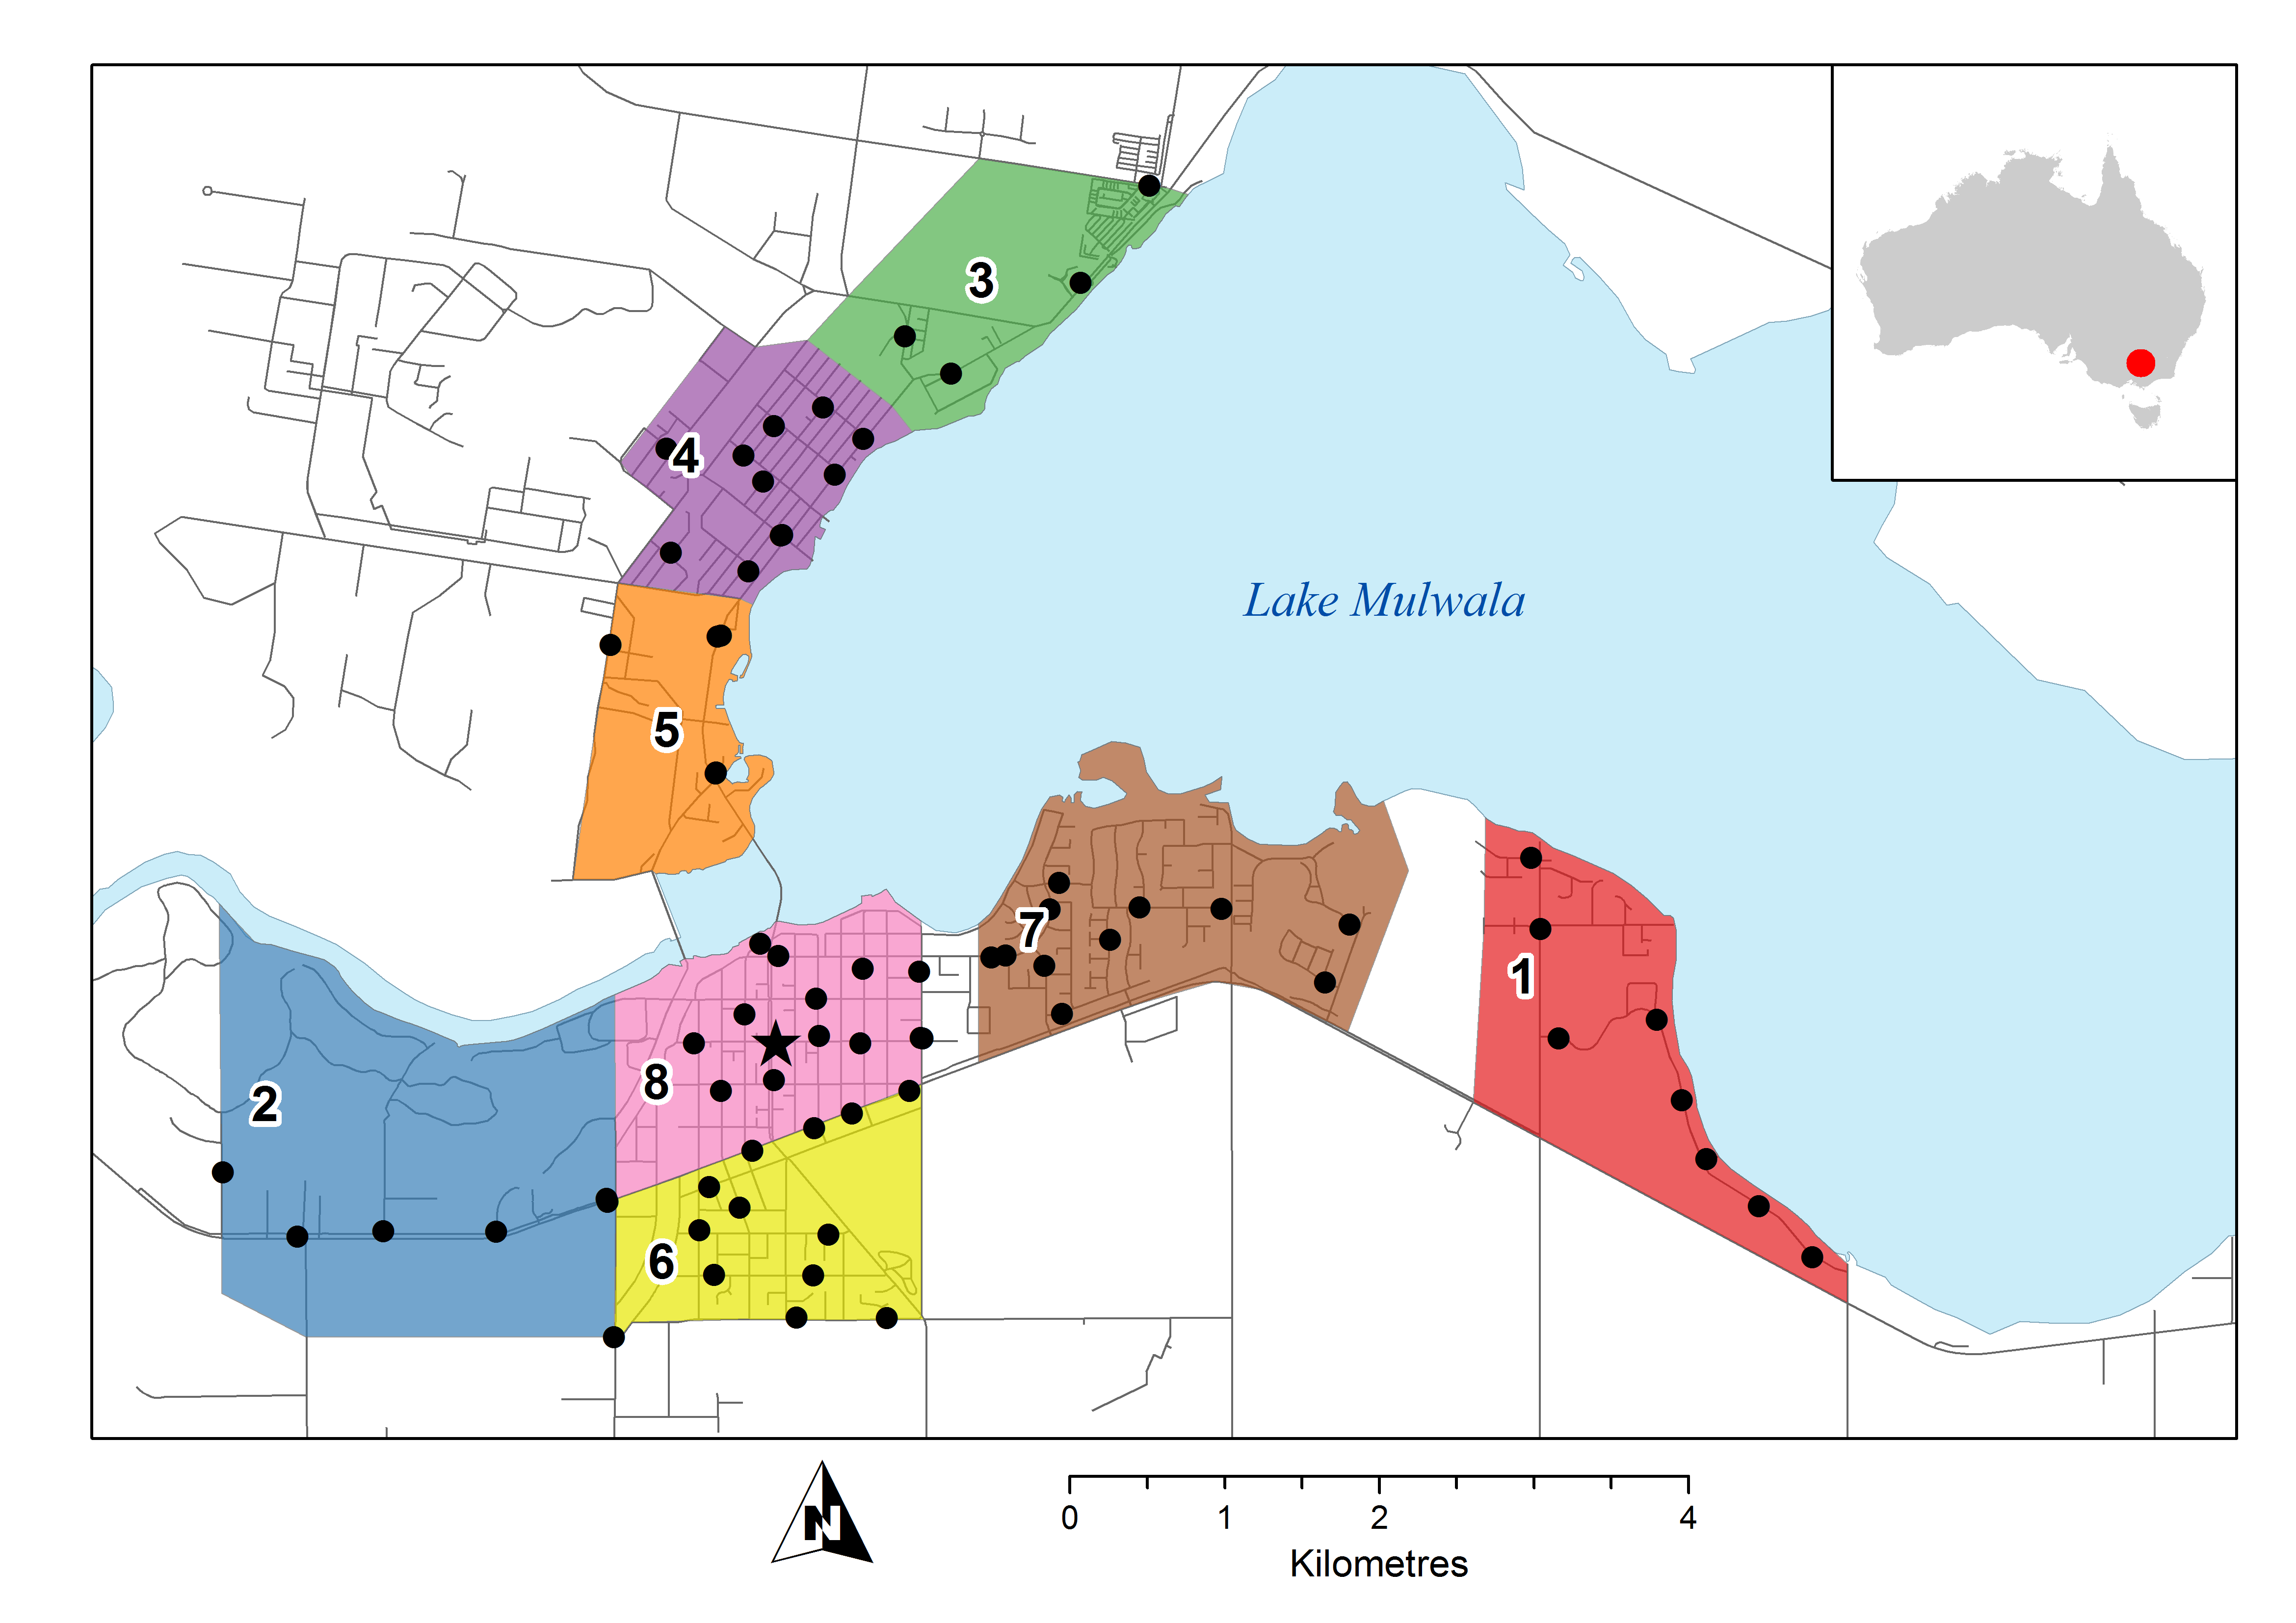
\includegraphics[width=0.85\textwidth, angle=0]{./using/figures/yarrawonga_high.png}}%
{}
%
% --------

Flexiride drivers record the location of pickups and drop-offs for each service,
as well as fare revenue collected. Using this data, probabilities of trips
occurring between two zones were developed following the process in
\citet[][]{Deflorio_ITSIET_2011}. A continuous distribution of departure times was
derived from evenly spreading the demand for particular services to either side
of that service. 

% --------
%Activity Locations: not used

% --------
%Network:
The network was extracted from OpenStreetMap. Some bus stops were removed if they were assigned to the same link in MATSim, e.g.,\,stops on the same road between intersections.

% --------
%Modes:
Only passengers for the demand-responsive service are included. However, the use of MATSim for this initial model means that we can add in other modes for later versions.

% --------
%Calibration and validation: exploratory

% --------
%Simulation quality and achieved results:
This was an exploratory simulation, intended to demonstrate how DRT can be modeled for exploring viability and how different schemes can be compared.

Using MATSim, experimentation with varying demands, two different scheduling
algorithms, and an altered Flexiride service with more services was able to be
carried out. Outcomes such as drive time, vehicle-kilometers traveled, and
passenger wait time could be measured.

Results showed that the two schemes performed differently for operators and
passengers. Optimization schemes had little effect with low demands, while
seating requirements showed more variability in the ad-hoc scheme as demand
increased. Future work involves estimating costs of the two schemes for further
comparison.

This work has been supported by a grant from the Australian Research Council (LP120200130). We are also grateful to Michal Maciejewski for his assistance with the dvrp module (see Chapter~\ref{ch:dts}). Michael Rigby prepared the map of Yarrawonga and Mulwala.
% ==================================================================================================================